\begin{frame}
  \begin{PointSix}{Houskeeping}
    \begin{itemize}
      \item \alert{Ask and take picture from Plenum.}
      \item \alert{Geophysics at seminar 20.05.2022}
      \item \alert{Should we do linearly varying density from Ex?}
    \end{itemize}
  \end{PointSix}
\end{frame}


\begin{frame}
    \begin{PointSix}{Learning Goals}
      \alert{Learning goals today:}
      \begin{itemize}
        \item Understand the shape of the magnetic anomalies
        \item Understand the measurement principle and sensors
        \item Understand different types of magnetism and its temperature dependency
      \end{itemize}
    \end{PointSix}
\end{frame}

\begin{frame}
  \begin{PointSix}{Remember: Differentiation between $\vec{H}$ and $\vec{B}$}
  The total (physically relevant) magnetic induction $\vec{B}$ is the superposition of external ($\vec{H}$) and local ($\chi \vec{M}$):
  \begin{align*}
    \vec{B} &= \mu_0\left(\vec{H} + \vec{M} \right)\\
            &= \mu_0 (1 + \chi) \vec{H} \\
            &= \mu_0 \mu \vec{H}
  \end{align*}
  $\mu \qquad \text{\small magnetic permeability}$
  $\chi \qquad \text{\small magnetic susceptibility (dimensionless)}$
  $[B]: \qquad \text{\small Tesla}$
  \end{PointSix}
\end{frame}

\begin{frame}
  \begin{PointSix}{Remember: Differentiation between $\vec{H}$ and $\vec{B}$}
  \alert{In geomagnetics, the magnetic susceptibility is the parameter that we are after.}
  \begin{align*}
    \vec{B} &= \mu_0\left(\vec{H} + \vec{M} \right)\\
            &= \mu_0 (1 + \chi) \vec{H} \\
            &= \mu_0 \mu \vec{H}
  \end{align*}
  $\mu \qquad \text{\small magnetic permeability}$
  $\chi \qquad \text{\small magnetic susceptibility (dimensionless)}$
  $[B]: \qquad \text{\small Tesla}$
  \end{PointSix}
\end{frame}

\begin{frame}
  \begin{PointSix}{Principals of magnetic surveys}
    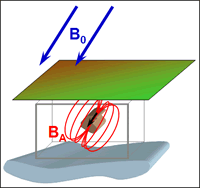
\includegraphics[width=0.80\linewidth]{Figures/Magnetics/inducing_field.png}

  \tiny [2017, GeoSci Developers.]
  \end{PointSix}
\end{frame}

\begin{frame}
  \begin{PointSix}{Principals of magnetic surveys}
    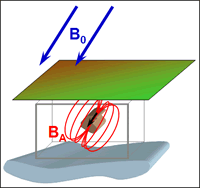
\includegraphics[width=0.80\linewidth]{Figures/Magnetics/inducing_field.png}

  \tiny [2017, GeoSci Developers.]
  \end{PointSix}
\end{frame}

\begin{frame}
  \begin{PointSix}{Principals of magnetic surveys}
    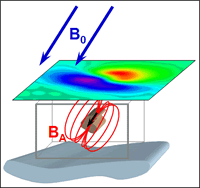
\includegraphics[width=0.80\linewidth]{Figures/Magnetics/magnetic_anomaly.png}

  \tiny [2017, GeoSci Developers.]
  \end{PointSix}
\end{frame}

\begin{frame}
  \begin{PointSix}{Principals of magnetic surveys}
    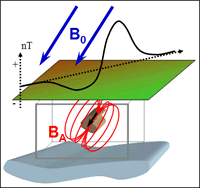
\includegraphics[width=0.80\linewidth]{Figures/Magnetics/measurements.png}

  \tiny [2017, GeoSci Developers.]
  \end{PointSix}
\end{frame}



\begin{frame}
    \begin{PointSix}{Strategy for expectations of induced magentic dipoles}
      \alert{Induced magnetic dipole:=Direction of $\vec{m} \parallel \vec{B}_0$}
      \small
      \begin{itemize}
        \item Draw S-End, N-End and inclination of planned profile
        \item Draw $\vec{m}$ and corresponding dipole field at depth
        \item Analyse superposition of $B_0$ and dipolfield. 
        \item (Assume that the anomaly is essentially parallel to $B_0$)
      \end{itemize}
    \end{PointSix}
\end{frame}

\begin{frame}
  \begin{PointSix}{Induced magnetization examples}
    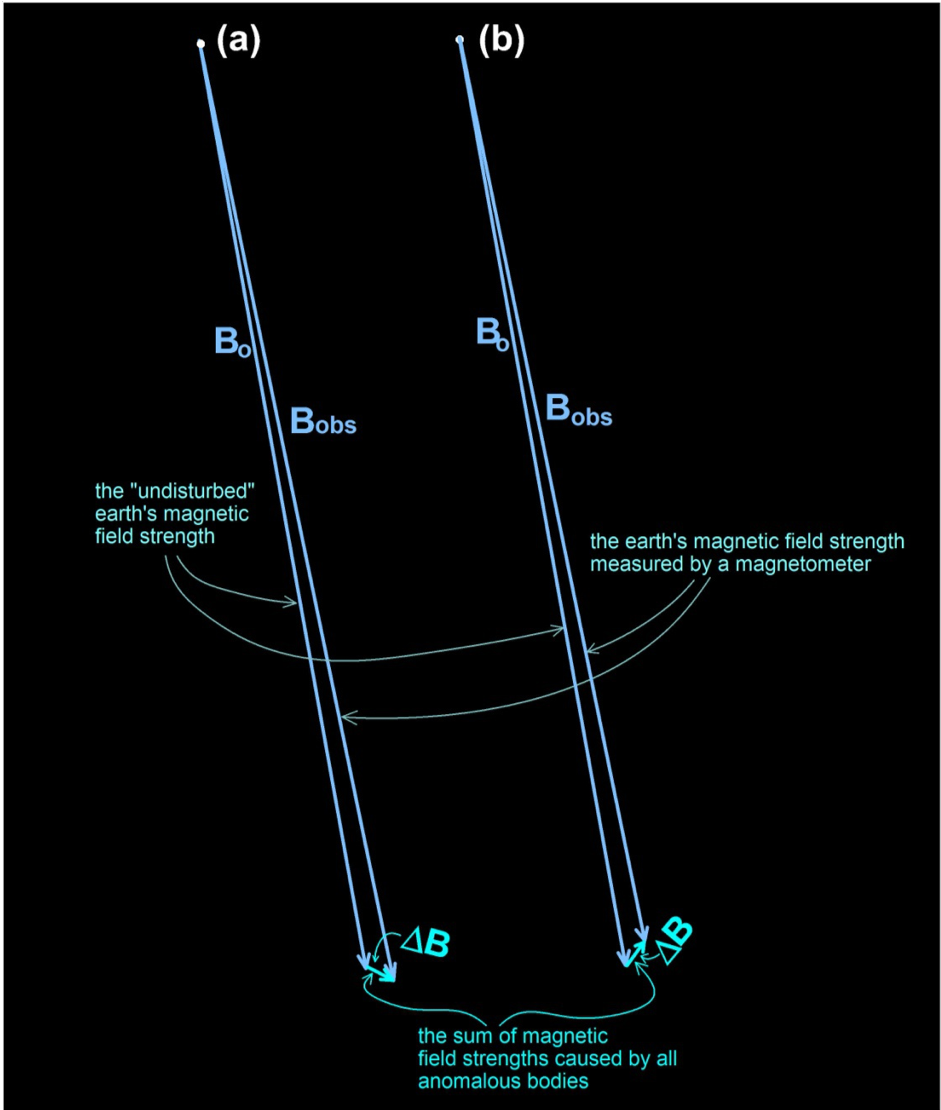
\includegraphics[width=0.7\textwidth]{Figures/Magnetics/AlmostParallel.png}

    [Soengonkono Intect 2015)]
  \end{PointSix}
\end{frame}

\begin{frame}
    \begin{PointSix}{Induced magnetization examples}
      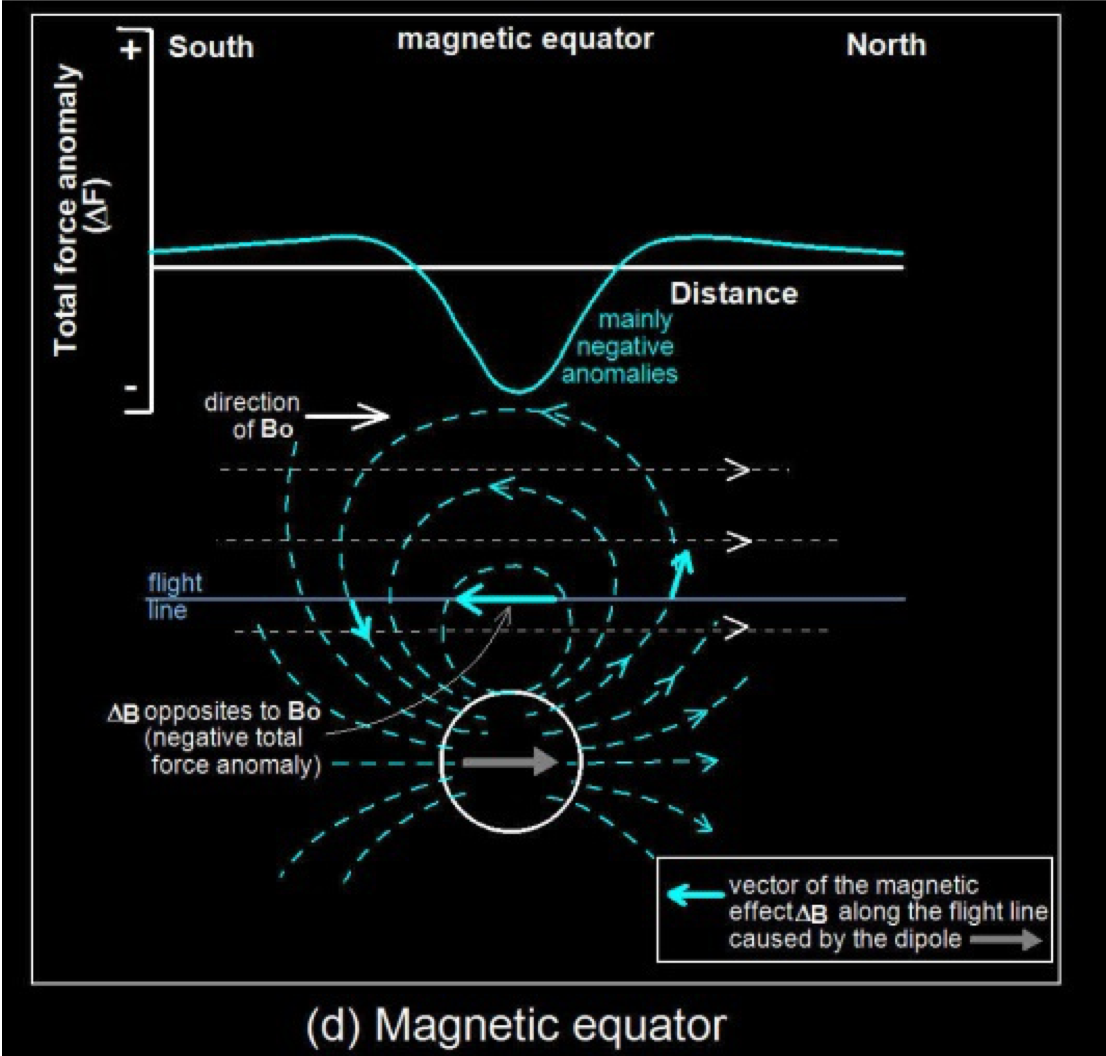
\includegraphics[width=0.9\textwidth]{Figures/Magnetics/AnomalyMagneticEquator.png}

      [Soengonkono Intect 2015)]
    \end{PointSix}
\end{frame}

\begin{frame}
    \begin{PointSix}{Induced magnetization examples}
      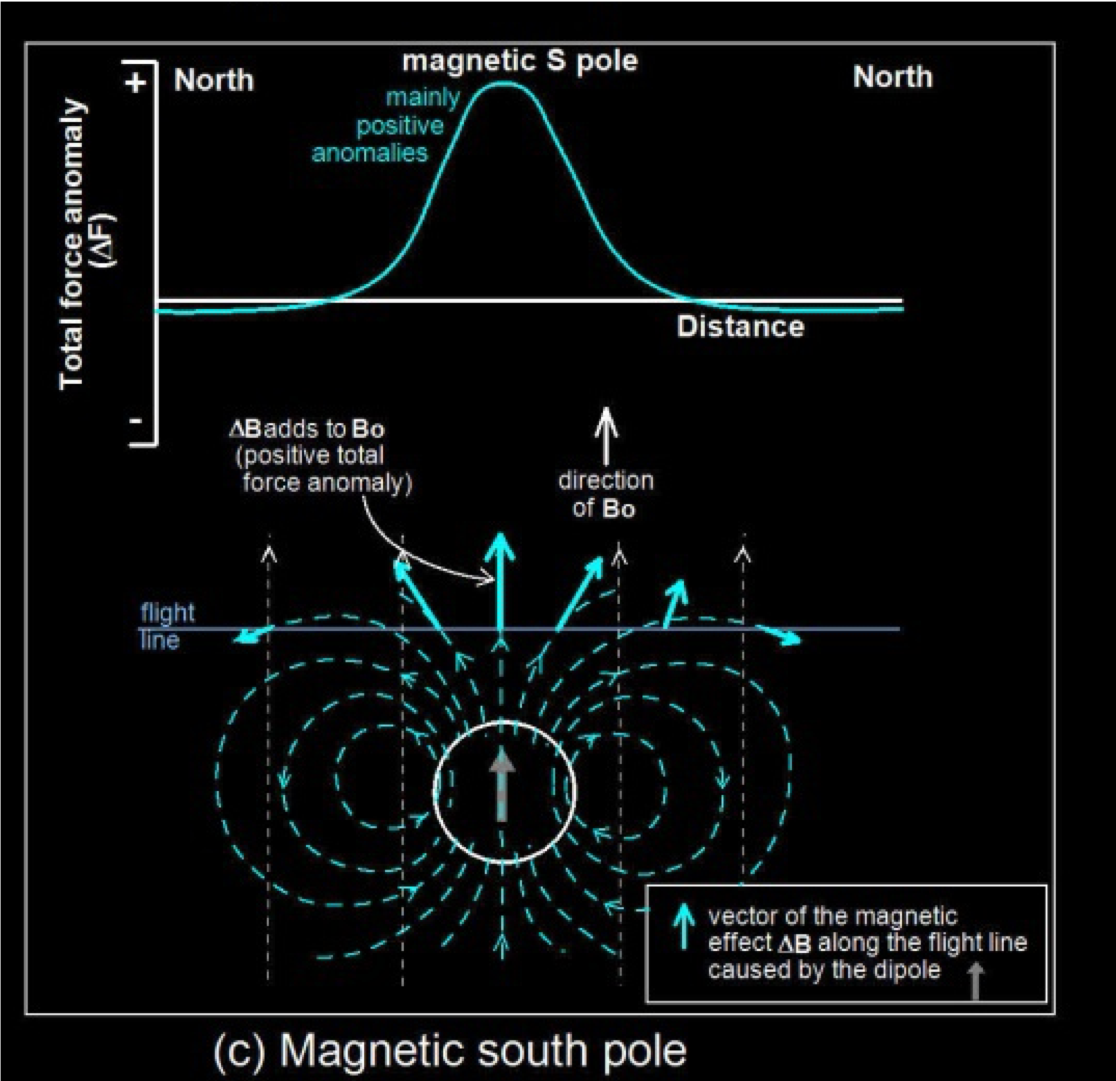
\includegraphics[width=0.9\textwidth]{Figures/Magnetics/AnomalyMagneticSouthPole.png}

      [Soengonkono Intect 2015)]
    \end{PointSix}
\end{frame}

\begin{frame}
    \begin{PointSix}{Induced magnetization examples}
      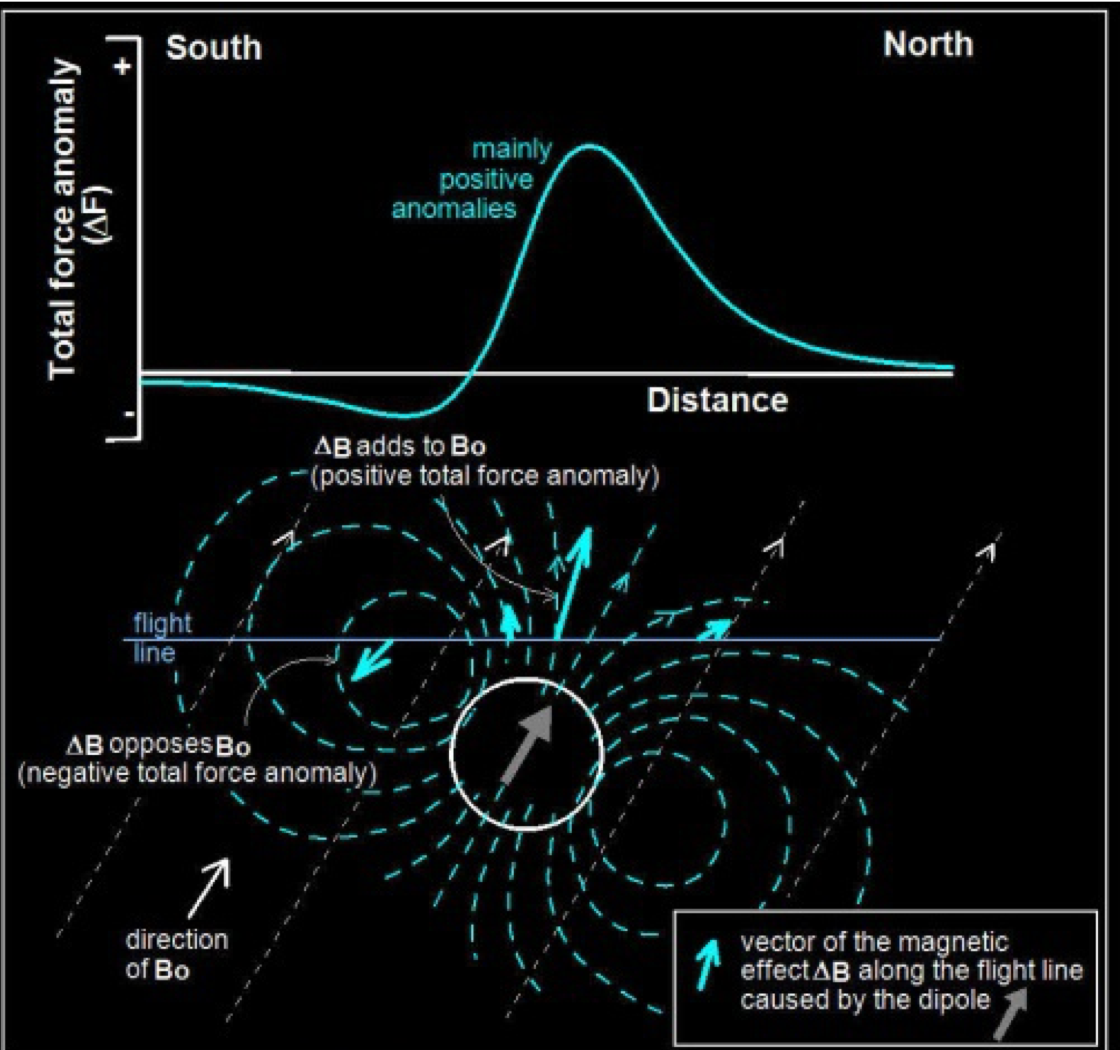
\includegraphics[width=0.9\textwidth]{Figures/Magnetics/AnomalySouthernHemisphere.png}

      [Soengonkono Intect 2015)]
    \end{PointSix}
\end{frame}

\begin{frame}
    \begin{PointSix}{Induced magnetization examples}
      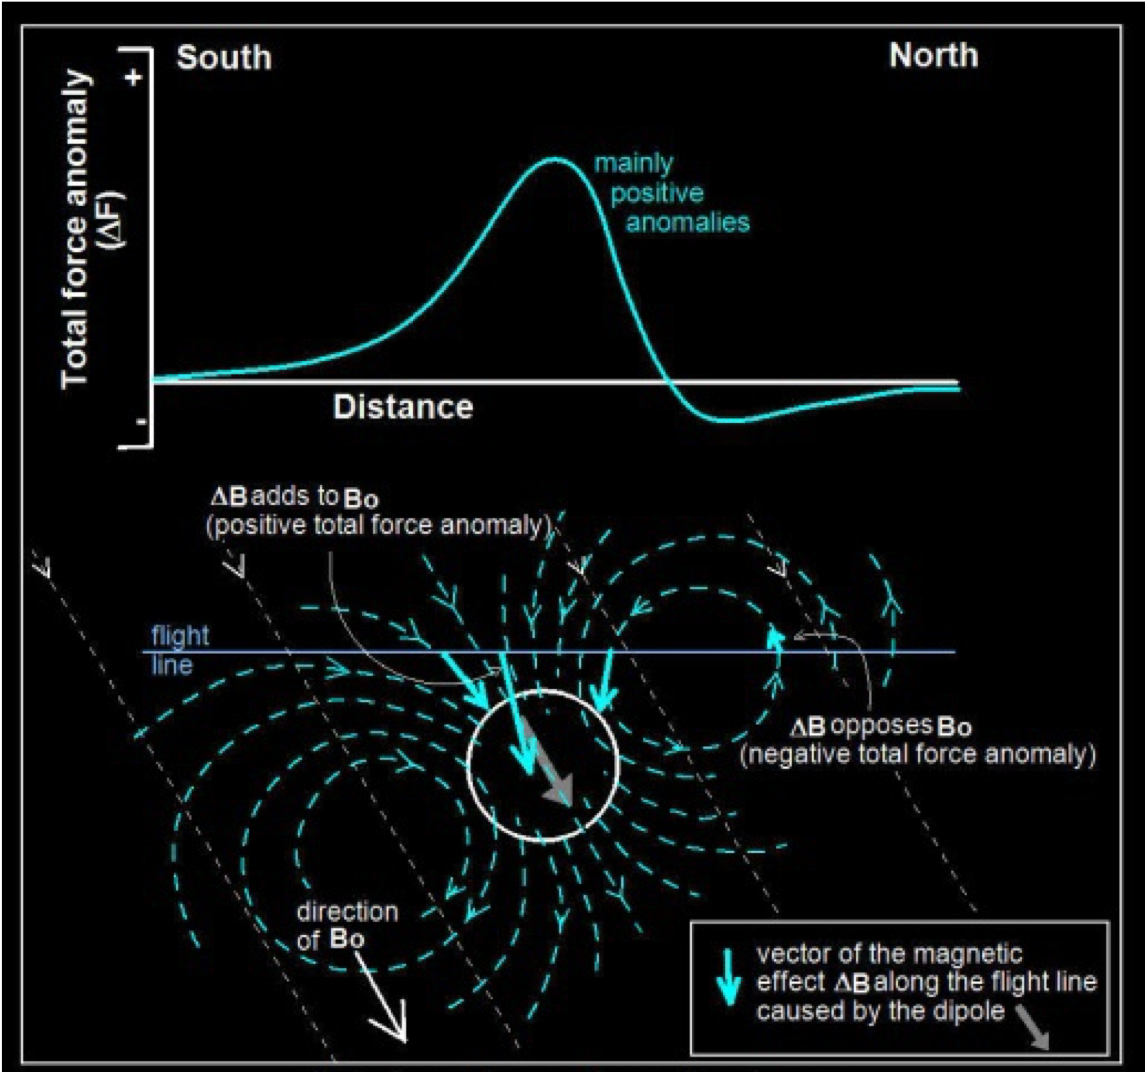
\includegraphics[width=0.9\textwidth]{Figures/Magnetics/AnomalyNothernHemisphere.png}

      [Soengonkono Intect 2015)]
    \end{PointSix}
\end{frame}

\begin{frame}
  \begin{PointSix}{Interpreting magnetic anomalies:}
    \begin{itemize}
      \item Unlike in gravity, magnetic can be measured in 3D
      \item Interpretation of $\Delta T$, $\Delta H$, $\Delta Z$, ...
      \item Commonly also the vertical gradient of $\Delta Z$ (cf. exercises)
    \end{itemize}
  \end{PointSix}
\end{frame}

\begin{frame}
  \begin{PointSix}{Demonstration of foreward model}
    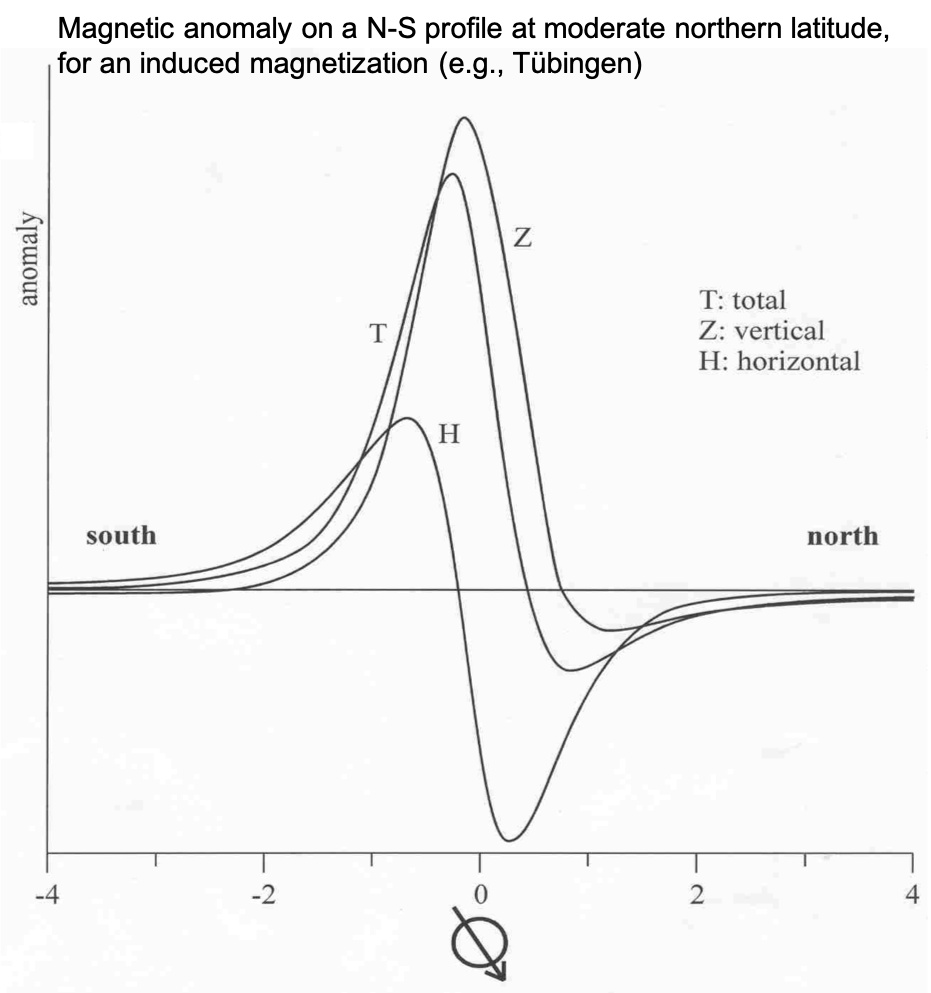
\includegraphics[width=0.9\textwidth]{Figures/Magnetics/MagneticAnomalyAllComponents.png}


  \end{PointSix}
\end{frame}


\begin{frame}
  \begin{PointSix}{Demonstration of foreward model}
    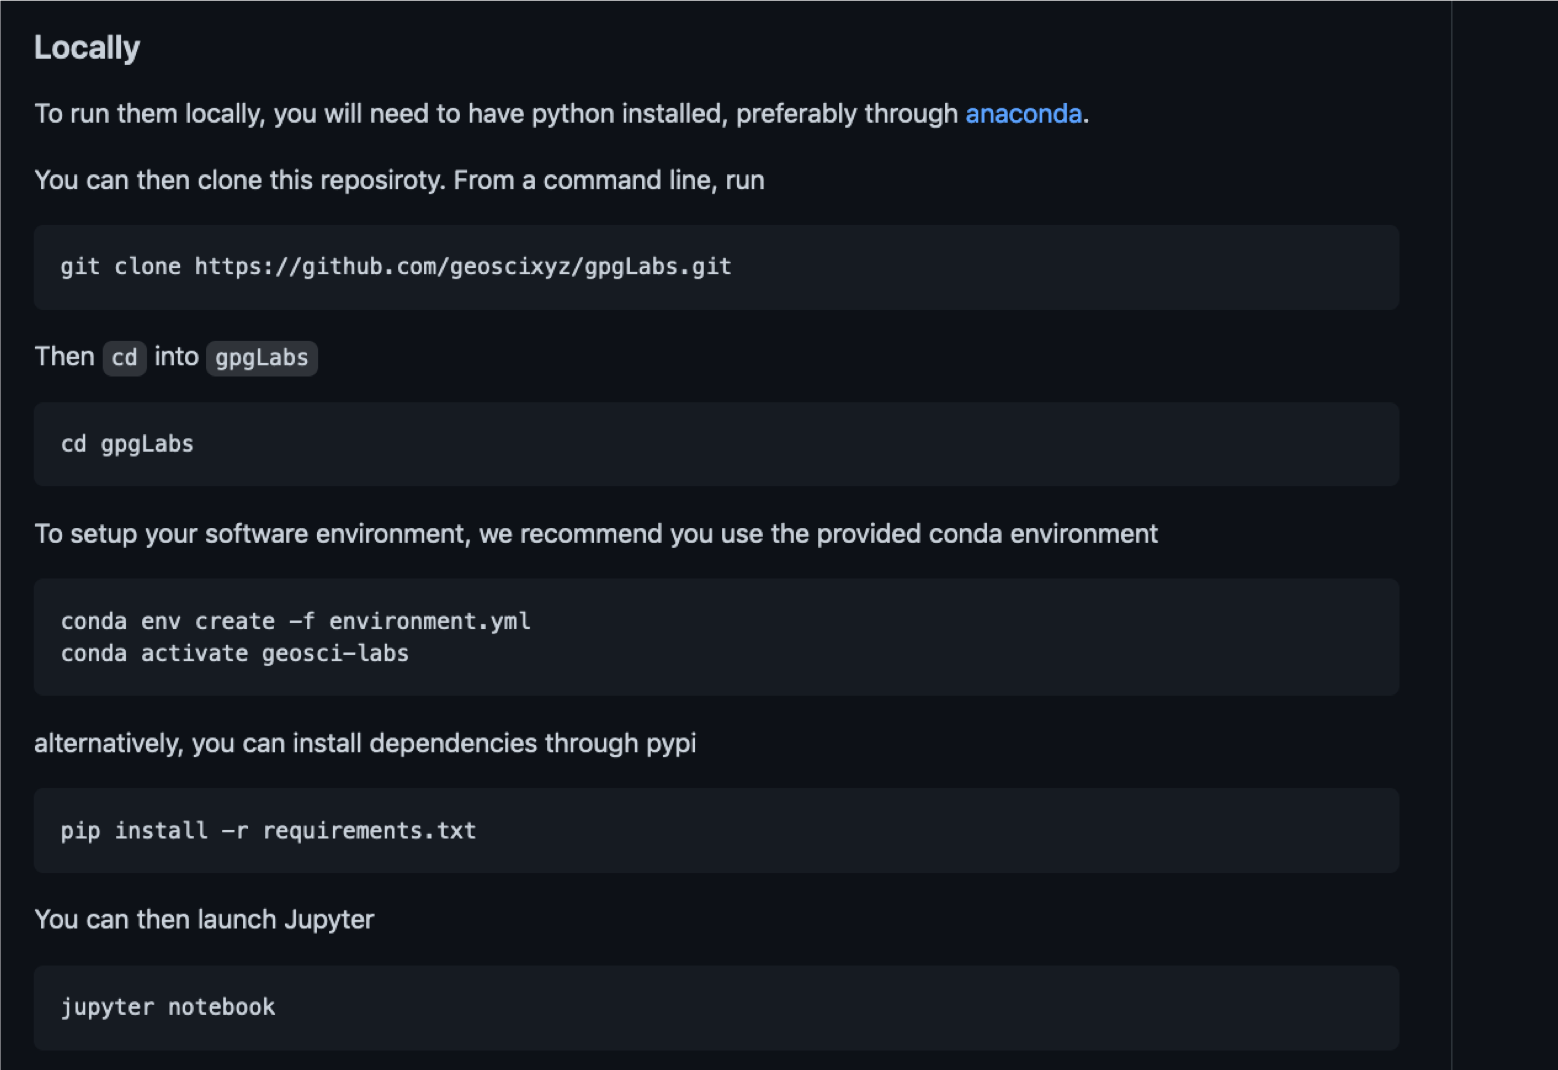
\includegraphics[width=0.9\textwidth]{Figures/Magnetics/GeoXYZ_Setup.png}


  \end{PointSix}
\end{frame}

\begin{frame}
  \begin{PointSix}{Demonstration of foreward model}
    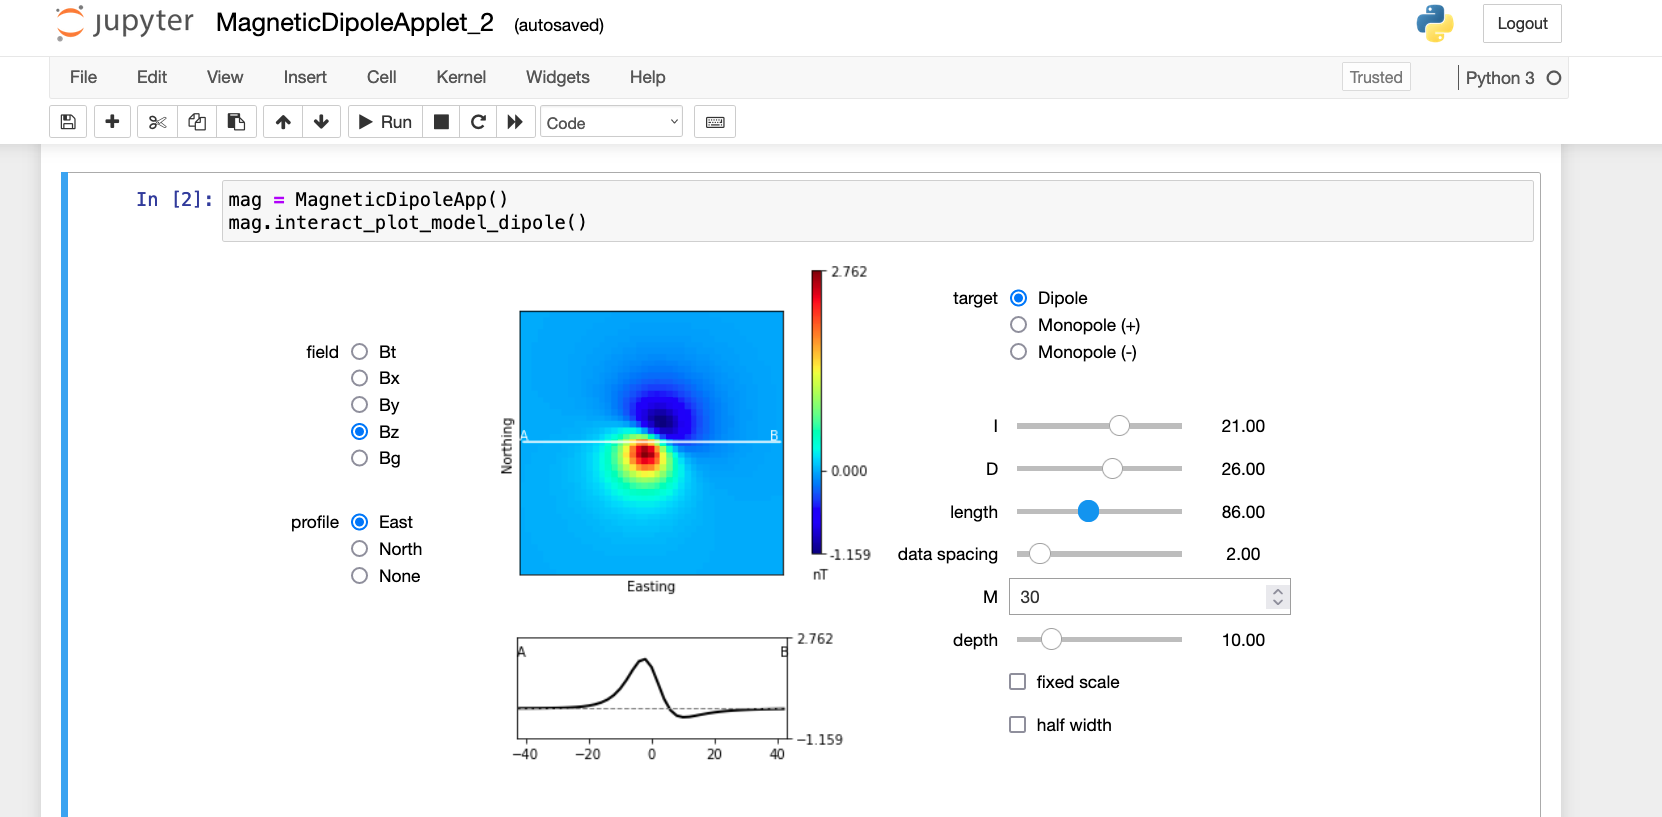
\includegraphics[width=0.9\textwidth]{Figures/Magnetics/GeosciXYZ_MagneticApplet.png}


  \end{PointSix}
\end{frame}

\begin{frame}
  \begin{PointSix}{Half-width rules}
   Similar to the anomaly in gravity surveys, we can also apply a half-width rule in magnetics to estimate the depth of the object. 

   $$
    d \sim HW
   $$

   Check this with the forward model.
  \end{PointSix}
\end{frame}







\begin{frame}
  \begin{PointSix}{Types of Magnetometers: Proton Precession}
    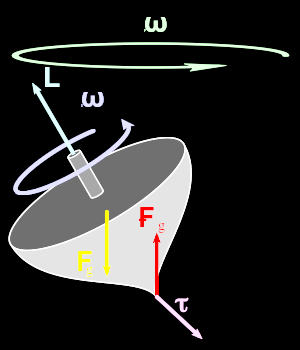
\includegraphics[width=0.8\textwidth]{Figures/Magnetics/LamorPrecession_XSnelgrove.png}

    \tiny [XSnelgrove (CC-BY-SA 2.5)]
  \end{PointSix}
\end{frame}

\begin{frame}
  \begin{PointSix}{Types of Magnetometers: Proton Precession}
  \small
    \begin{itemize}
      \item Hydrogen atoms have angular momentum (spin) and magnetic moment (moved charge). Both are vectors which are parallel to each other and linked by the gyromagnetic ratio ($\gamma_p$).
    \end{itemize}
  \end{PointSix}
\end{frame}

\begin{frame}
  \begin{PointSix}{Types of Magnetometers: Proton Precession}
    \small
    \begin{itemize}
      \item Protons have angular momentum and magnetic moment.
      \item External magnetic field induces torque, so that mini magnetic moment tends to aligns parallel to the external field.
    \end{itemize}
  \end{PointSix}
\end{frame}

\begin{frame}
  \begin{PointSix}{Types of Magnetometers: Proton Precession}
    \small
    \begin{itemize}
      \item Hydrogen atoms have angular momentum and magnetic moment.
      \item External magnetic field induces torque, alignment near parallel to external field.
      \item Because of internal spin, this torque induces precession (analogy to spinning top).
    \end{itemize}
  \end{PointSix}
\end{frame}

\begin{frame}
  \begin{PointSix}{Types of Magnetometers: Proton Precession}
    \small
    \begin{itemize}
      \item Hydrogen atoms have angular momentum and magnetic moment.
      \item External magnetic field induces torque, alignment near parallel to external field.
      \item Because of internal spin, this torque induces precession (analogy to spinning top).
      \item The precession frequency $\omega$ is sensitive to the \textit{total external field}, not its direction. 
    \end{itemize}
    $$
      \omega = \gamma_p |B|
    $$
  \end{PointSix}
\end{frame}

\begin{frame}
  \begin{PointSix}{Types of Magnetometers: Proton Precession}
    \small
    \begin{itemize}
      \item Hydrogen atoms have angular momentum and magnetic moment.
      \item External magnetic field induces torque, alignment near parallel to external field.
      \item Because of internal spin, this torque induces precession (analogy to spinning top).
      \item The precession frequency $\omega$ is sensitive to the \textit{total external field}, not its direction. 
      \item \alert{Idea: Measure $\omega$ and infer $|B|$}
    \end{itemize}
    $$
      \omega = \gamma_p |B|
    $$
  \end{PointSix}
\end{frame}

\begin{frame}
  \begin{PointSix}{Types of Magnetometers: Proton Precession}
    \small
    \alert{Practical implementation:}
    \begin{itemize}
      \item Use liquid with many hydrogen atoms (e.g. water or kerosene).
      \item Align their magnetic moments with strong, external magnetic field.
    \end{itemize}
  \end{PointSix}
\end{frame}


\begin{frame}{Types of Magnetometers: Fluxgate}
  %\begin{PointSix}{Induced magnetization examples}
    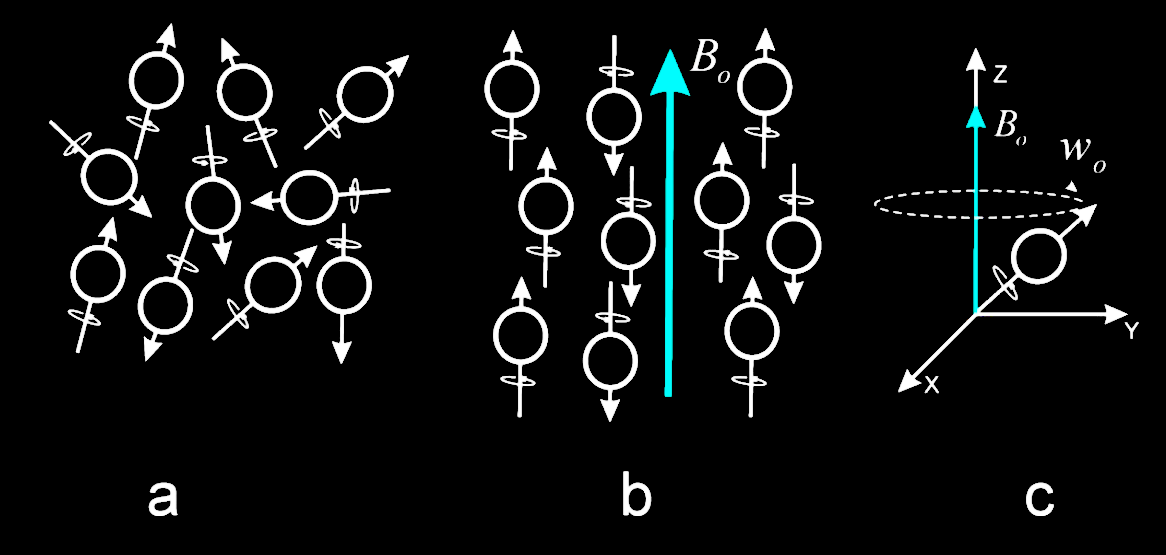
\includegraphics[width=0.8\textwidth]{Figures/Magnetics/ProtonPrecessionSpinAlignment_FOrdonez2014.png}
    
    \tiny [F. Ordonez 2014]

    \alert{\small At room temperatures spins are not aligned as Earth's magnetic field is too weak to do so.}
  %\end{PointSix}
\end{frame}

\begin{frame}
  \begin{PointSix}{Types of Magnetometers: Proton Precession}
    \small
    \alert{Practical implementation:}
    \begin{itemize}
      \item Use liquid with many hydrogen atoms (e.g. water or kerosene).
      \item Align their magnetic moments with strong, external magnetic field.
      \item Measure the precession frequency (how?)
    \end{itemize}
  \end{PointSix}
\end{frame}

\begin{frame}{Induction: Time variable $B$ field induce currents}
  \centering
  \animategraphics[loop,width=9cm]{10}{Figures/Magnetics/animation/Electromagnetic_induction_Ponor-}{0}{20}

  \tiny [Animation by Ponor (CC-BY-SA)]
\end{frame}

\begin{frame}{Induction: Time variable $B$ field induce currents}
  $$
    \varepsilon = \frac{d\phi_B}{dt}
  $$
  \begin{itemize}
    \item $\varepsilon$ electromotive force (e.g., leads to current in coil)
    \item $\phi_B$ intercepted magnetic flux 
  \end{itemize}

\end{frame}

\begin{frame}{Induction: Time variable $B$ field induce currents}
  $$
    \varepsilon = \frac{d\phi_B}{dt}
  $$
  \begin{itemize}
    \item $\varepsilon$ electromotive force (e.g., leads to current in coil)
    \item $\phi_B$ intercepted magnetic flux 
    \item Faraday's law of induction
  \end{itemize}
  $$
    \nabla \times \vec{E} = -\frac{\partial}{\partial t}\vec{B}
  $$

\end{frame}

\begin{frame}
  \begin{PointSix}{Types of Magnetometers: Proton Precession}
    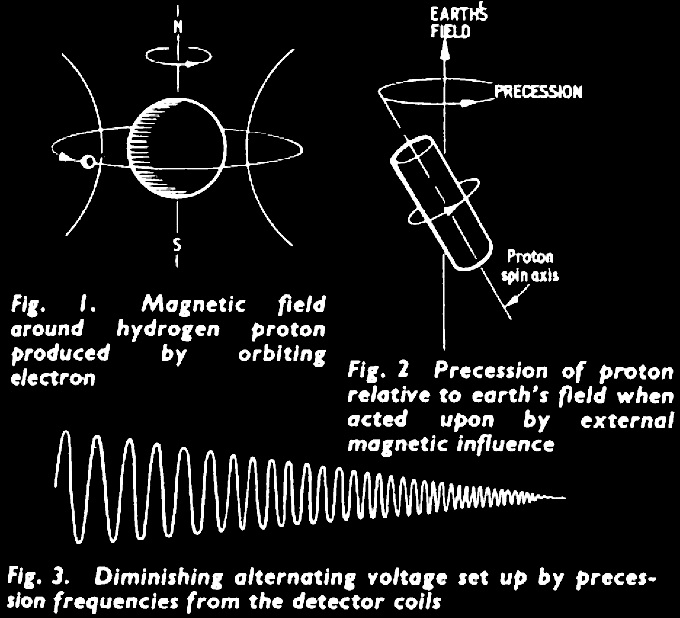
\includegraphics[width=0.85\textwidth]{Figures/Magnetics/ProtonPrecesssion_Huggard1970.jpg}

    \tiny [Huggard 1970]
  \end{PointSix}
\end{frame}

\begin{frame}
  \begin{PointSix}{Types of Magnetometers: Proton Precession}
    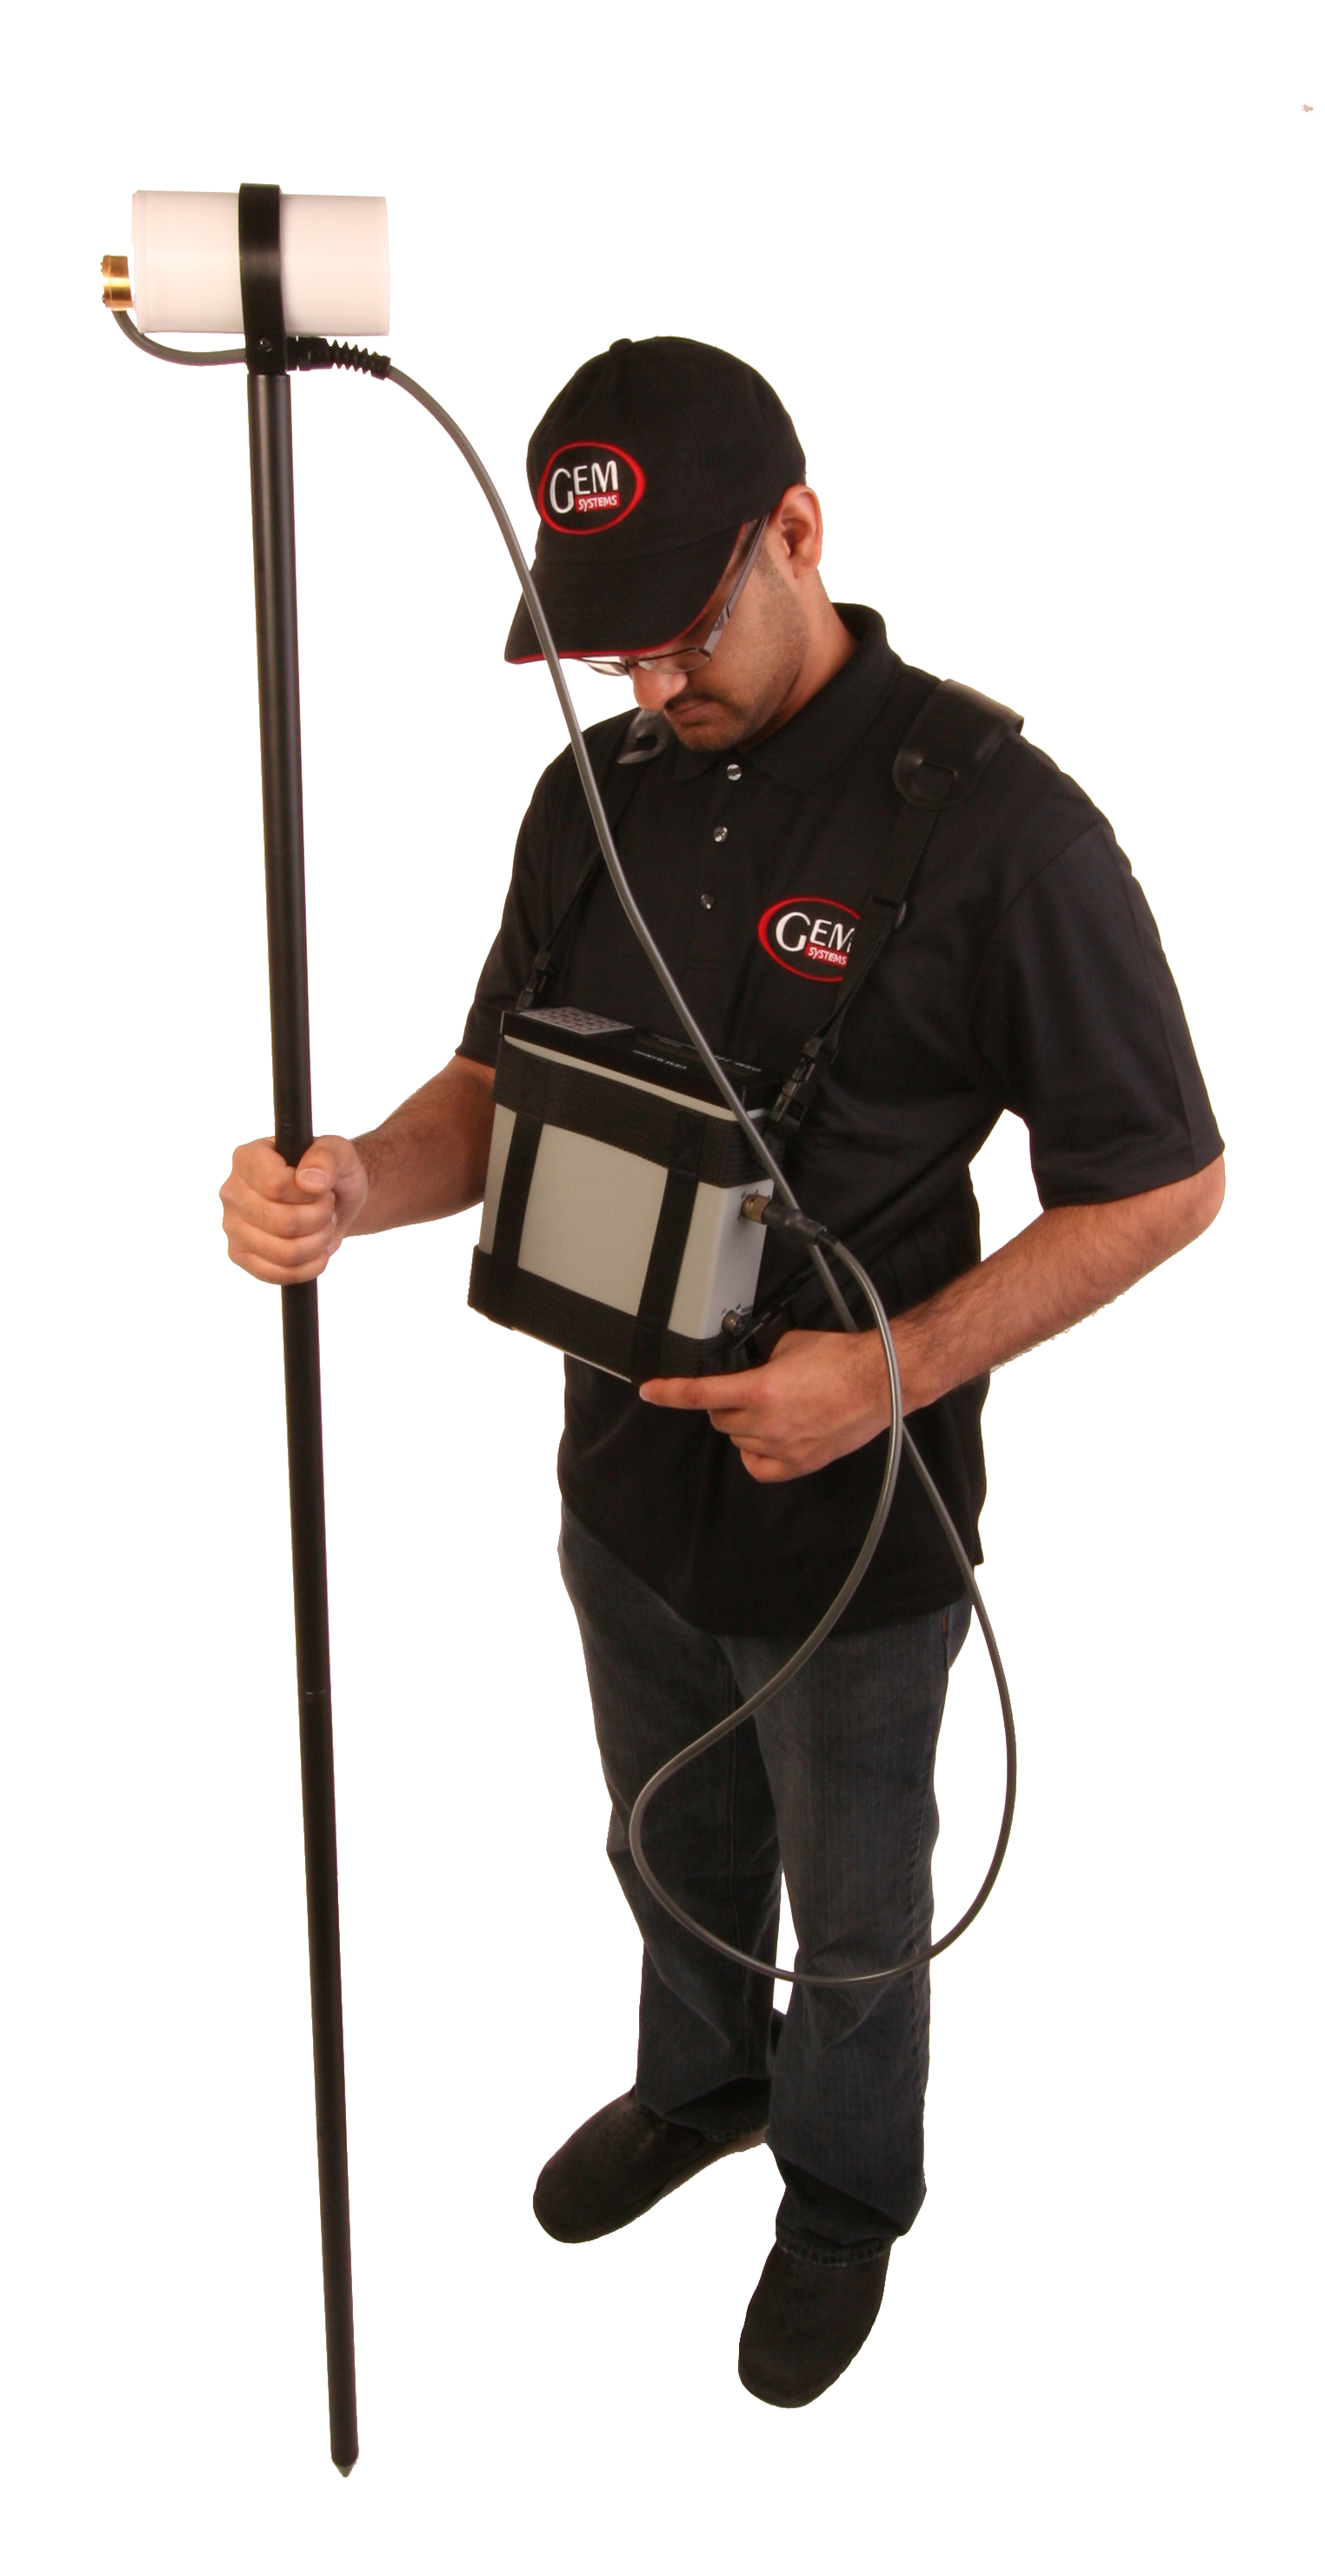
\includegraphics[width=0.5\textwidth]{Figures/Magnetics/ProtonPrecession_Gemsys2012.png}

    \tiny [Gemsys 2012]
  \end{PointSix}
\end{frame}

\begin{frame}
  \begin{PointSix}{Types of Magnetometers: Proton Precession}
  \small
    \begin{itemize}
      \item Measures total field (alignment of sensor less important).
      \item Based on magnetic moment of hydrogen atom and larmor precession.
      \item Alignment in artificial external $B$ field.
      \item Measure relaxation and larmor precession via induction in surrounding coils.
      \item Sensitivity $\sim 0.1 nT$.
      \item Principals are similar to MRI
    \end{itemize}
  \end{PointSix}
\end{frame}



\begin{frame}{Types of Magnetometers: Fluxgate}
  % \begin{PointSix}{Induced magnetization examples}
     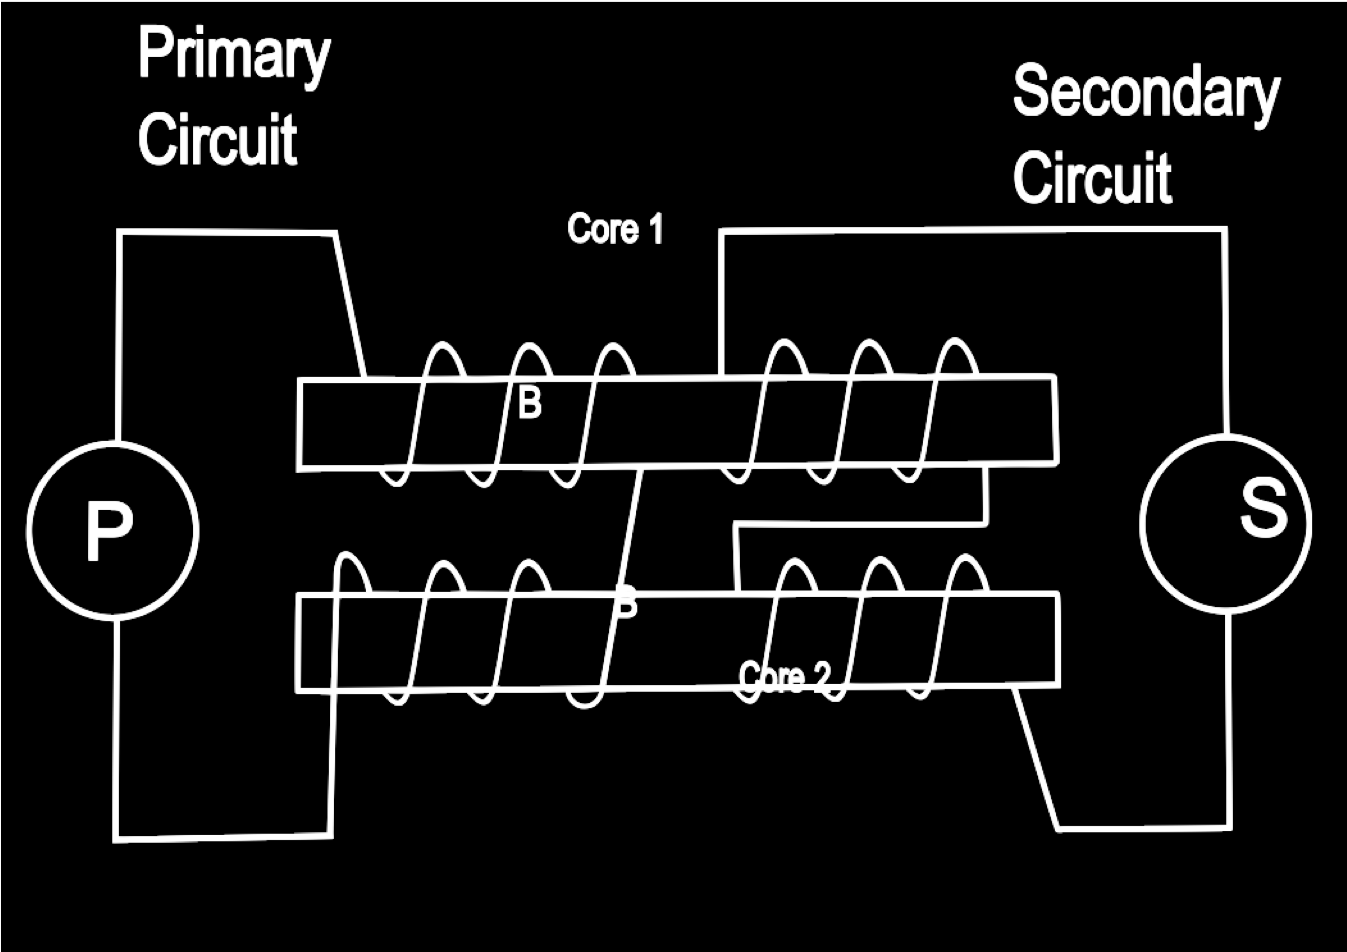
\includegraphics[width=0.8\textwidth]{Figures/Magnetics/Fluxgate_PDornelCCBYSA.png}
 
     \tiny [PDornel (CC-BY-SA)]
  % \end{PointSix}
 \end{frame}

 \begin{frame}
  \begin{PointSix}{Fluxgate magnetometer}
   \begin{itemize}
    \item Induce low-frequencey (kHz) current in primary circuit.
    \item The magnetic fields in secondary coil will be balanced \alert{in absence of external field.}
    \item External field causes imbalance between primary and secondary coils that can be used to measure $B_x$, $B_y$, $B_z$ \alert{depending on coil orientation.}
   \end{itemize}
  \end{PointSix}
\end{frame}


\begin{frame}{Types of Magnetometers: Fluxgate}
  \begin{tikzpicture}
    \node (fig1) at (0,0) {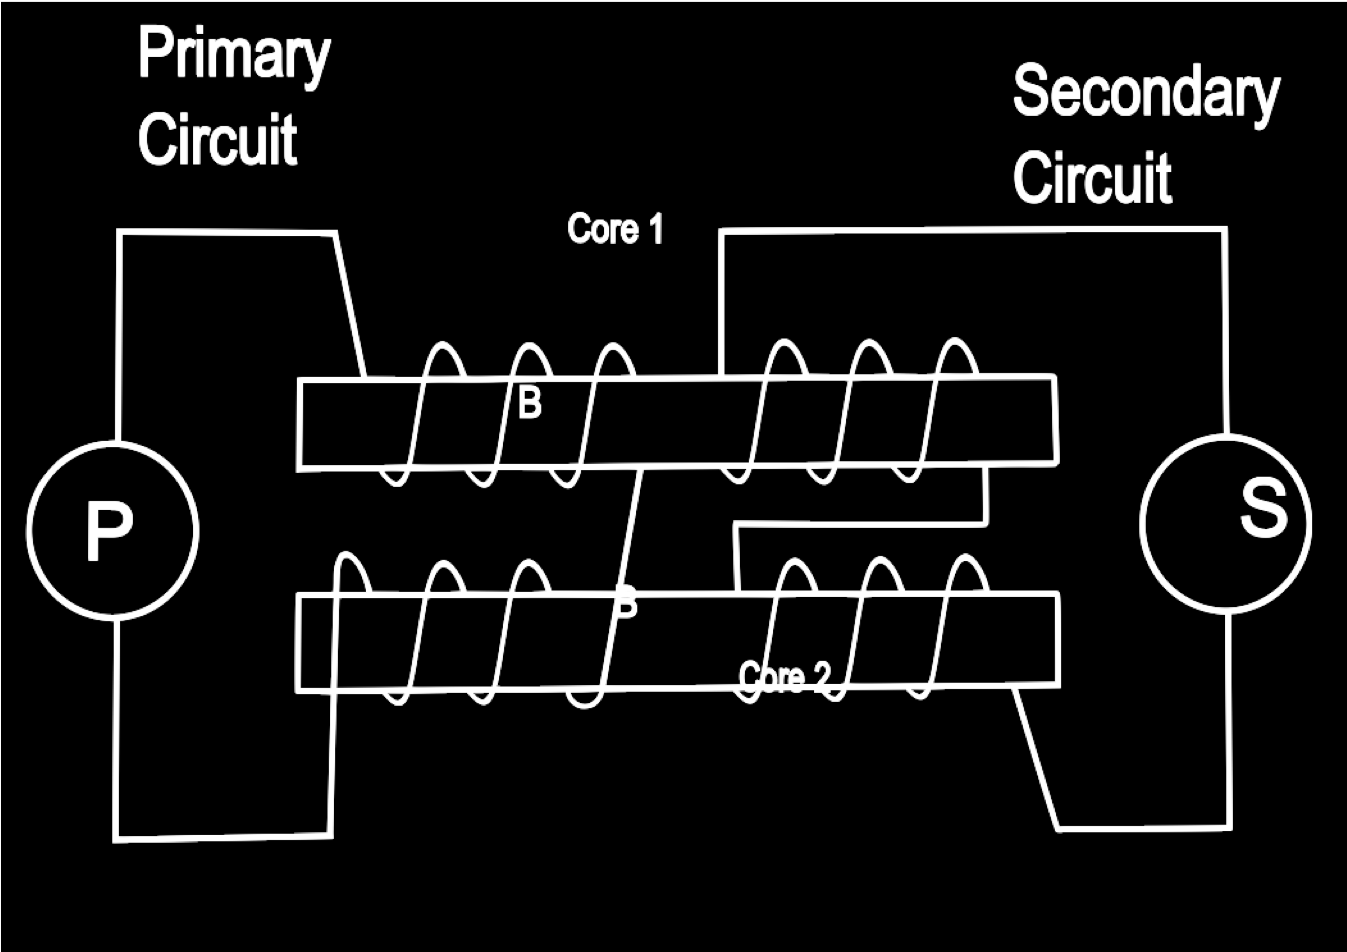
\includegraphics[scale=0.5]{Figures/Magnetics/Fluxgate_PDornelCCBYSA.png}};
    \draw [<-, line width=0.75mm, red](-3,0.6) -- (0,0.6);
    \draw [->, line width=0.75mm, red](-3,-1.5) -- (0,-1.5);
  \end{tikzpicture}
 \end{frame}

 \begin{frame}{Types of Magnetometers: Fluxgate}
  \begin{tikzpicture}
    \node (fig1) at (0,0) {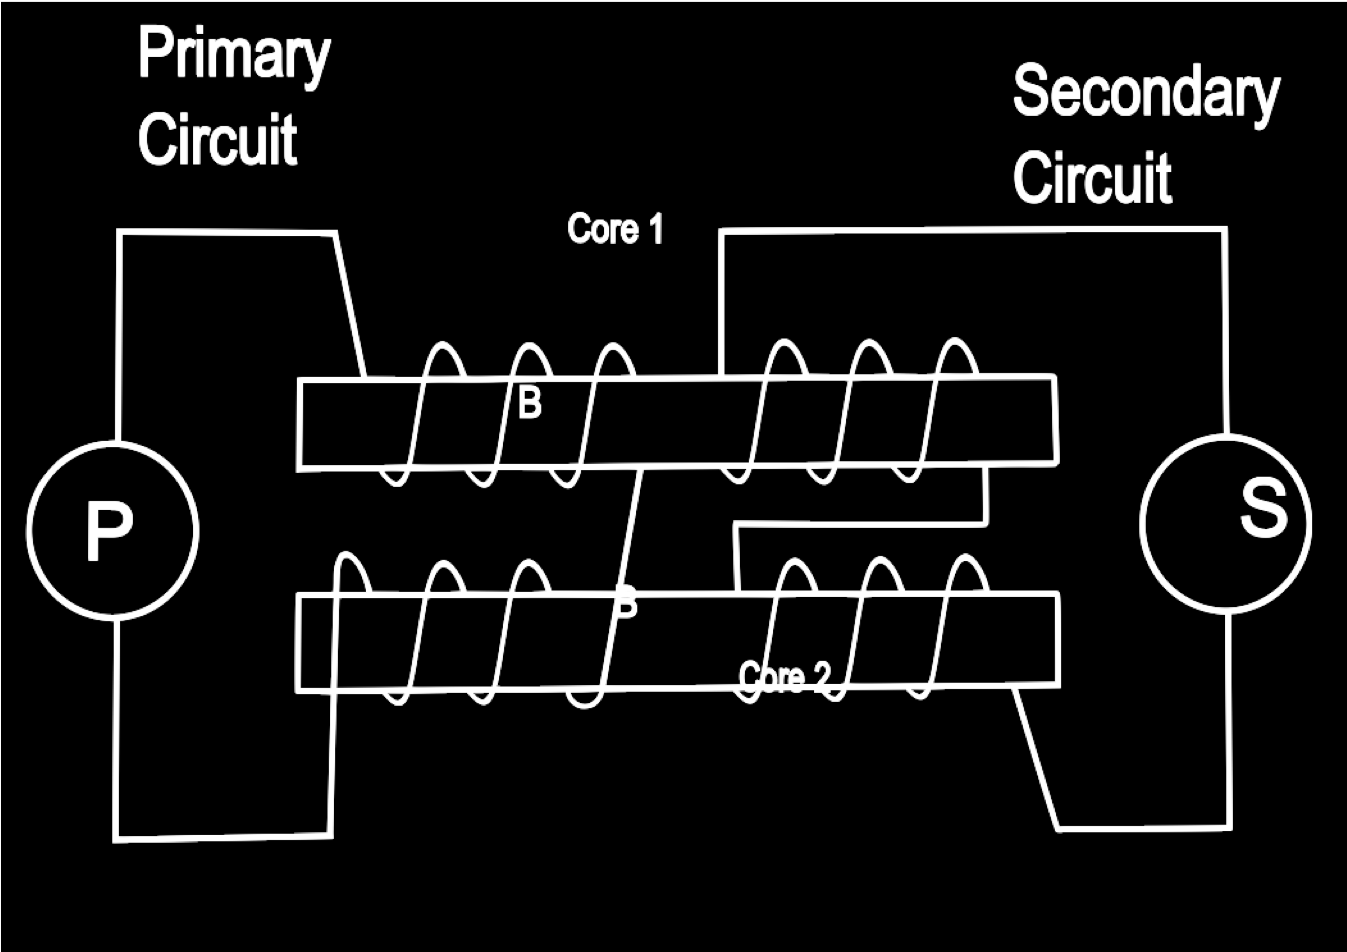
\includegraphics[scale=0.5]{Figures/Magnetics/Fluxgate_PDornelCCBYSA.png}};
    \draw [<-, line width=0.75mm, red](-3,0.6) -- (-0.5,0.6);
    \draw [->, line width=0.75mm, red](-3,-1.5) -- (0.5,-1.5);
    \draw [->, line width=0.75mm, blue](-3,3) -- (4,-3);
  \end{tikzpicture}
 \end{frame}

 \begin{frame}{Types of Magnetometers: Optically pumped}
  % \begin{PointSix}{Induced magnetization examples}
     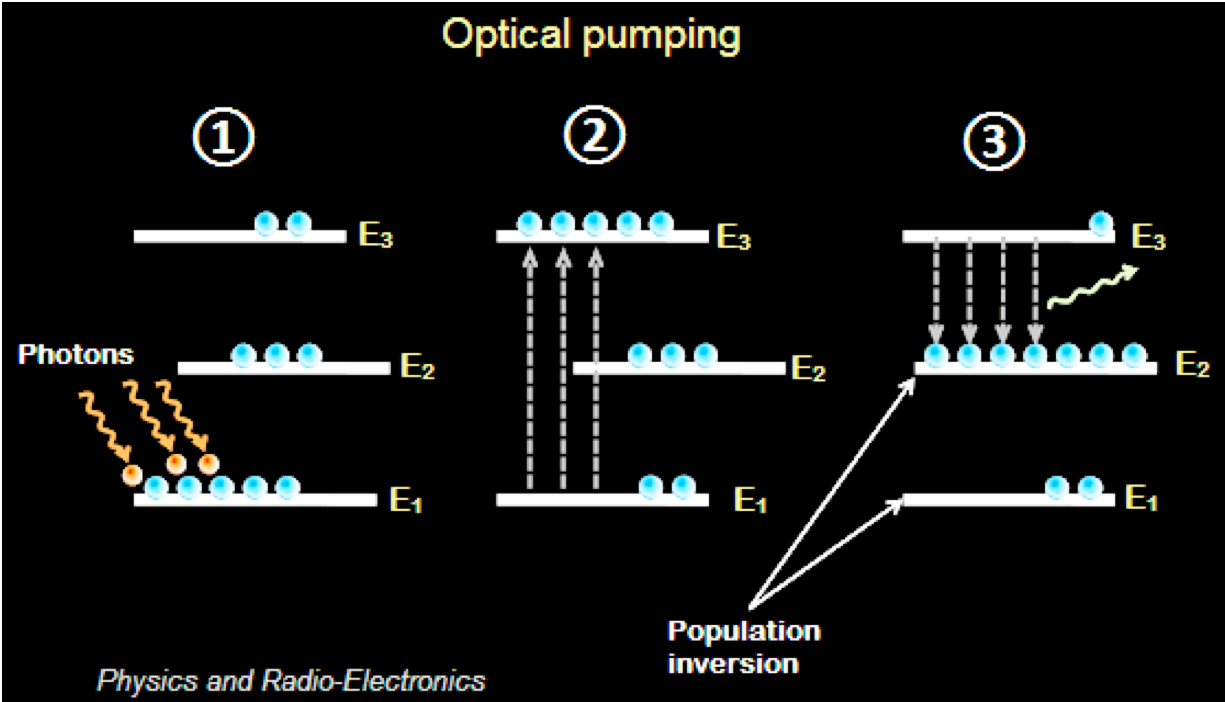
\includegraphics[width=0.8\textwidth]{Figures/Magnetics/OpticallyPumped_PDornel.png}
 
     \tiny [PDornel (CC-BY-SA)]
  % \end{PointSix}
 \end{frame}

\begin{frame}
  \begin{PointSix}{Gradiometry: Measure the vertical gradient}
   \begin{itemize}
    \item Install two sensors at different heights (e.g., 0.5 m apart).
    \item Consider only the vertical gradient.
    \item Insensitive to the total field and temporal variability thereof.
    \item Sensitive to near-surface structures (why?).
    \item Sensitive to horizontal boundaries.
    \item \alert{Relevant for applied exercises.}
   \end{itemize}
  \end{PointSix}
\end{frame}



\begin{frame}
  \begin{center}
    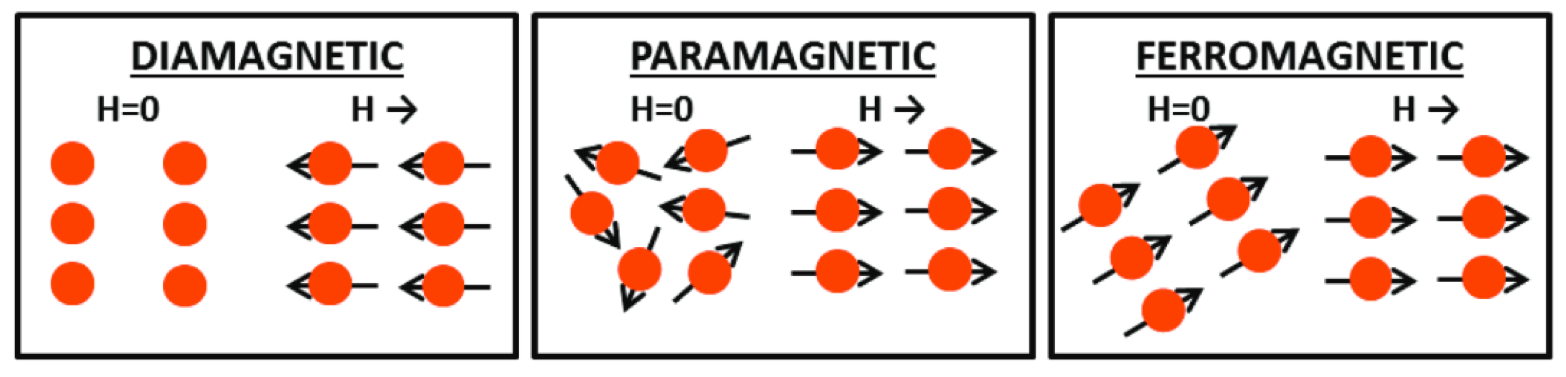
\includegraphics[width=0.7\linewidth]{Figures/Magnetics/ParaDiaFerro_Lacovacci2016.png}
  
    \tiny[Lacovacci2016]

    \vspace{2cm}
    
    \normalsize How do materials react to application of an external magnetic field?
  \end{center}
\end{frame}

\begin{frame}
  \begin{center}
    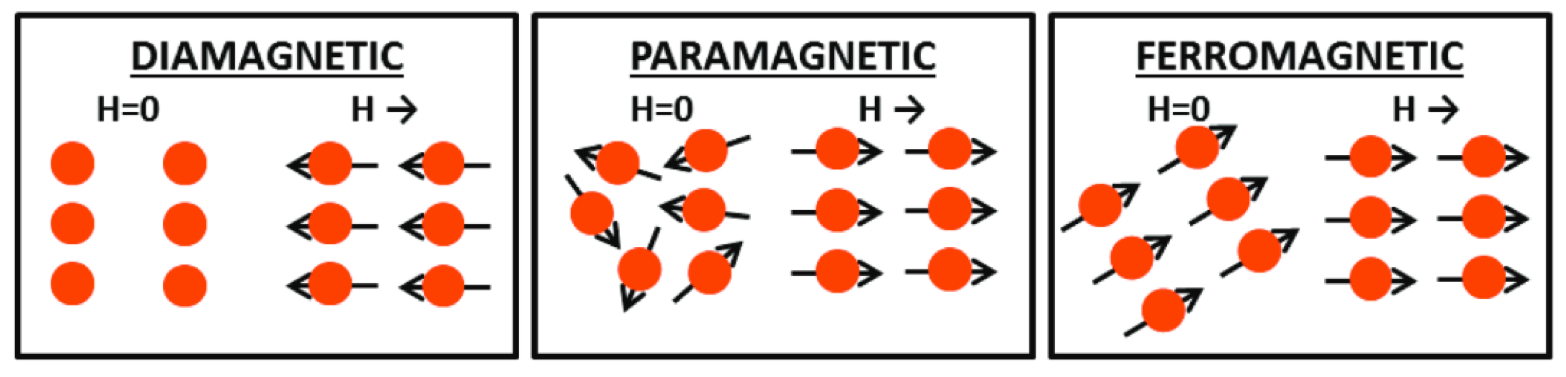
\includegraphics[width=0.7\linewidth]{Figures/Magnetics/ParaDiaFerro_Lacovacci2016.png}
  
    \tiny[Lacovacci2016]

    \vspace{0.24cm}
    
    \normalsize Diamagnetism
    \small 
    \begin{itemize}
      \item \alert{Weak} mini-dipoles induced, opposing external field ($\chi < 0$).
      \item Diappears if external field is removed.
      \item Occurs essentially in all materials, but is not noted everywhere, due to other effects. 
      \item Examples: Quarzite, Calcite, ...
    \end{itemize}
    
  \end{center}
\end{frame}

\begin{frame}
  \begin{center}
    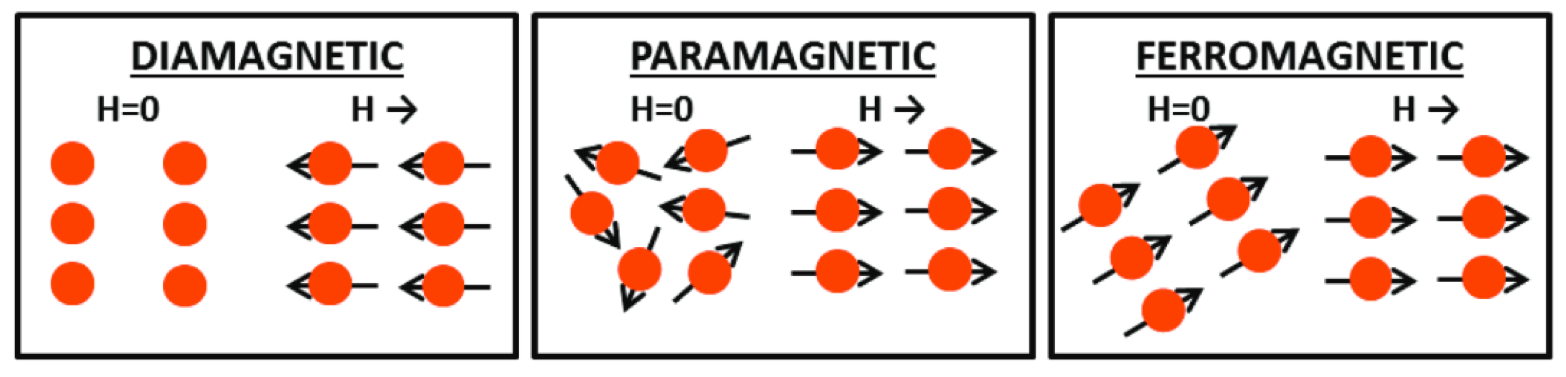
\includegraphics[width=0.7\linewidth]{Figures/Magnetics/ParaDiaFerro_Lacovacci2016.png}
  
    \tiny[Lacovacci2016]

    \vspace{0.24cm}
    
    \normalsize Paramagnetism
    \small 
    \begin{itemize}
      \item Material exhibits \alert{pre-existing} dipoles which orient themselves in external field (unpaired electrons).
      \item \alert{Reinforce} external field ($\chi > 0$). 
      \item Effect dissipates due to thermal fluctuations once external field is removed.
      \item Examples: gold, copper,...
    \end{itemize}
    
  \end{center}
\end{frame}

\begin{frame}
  \begin{center}
    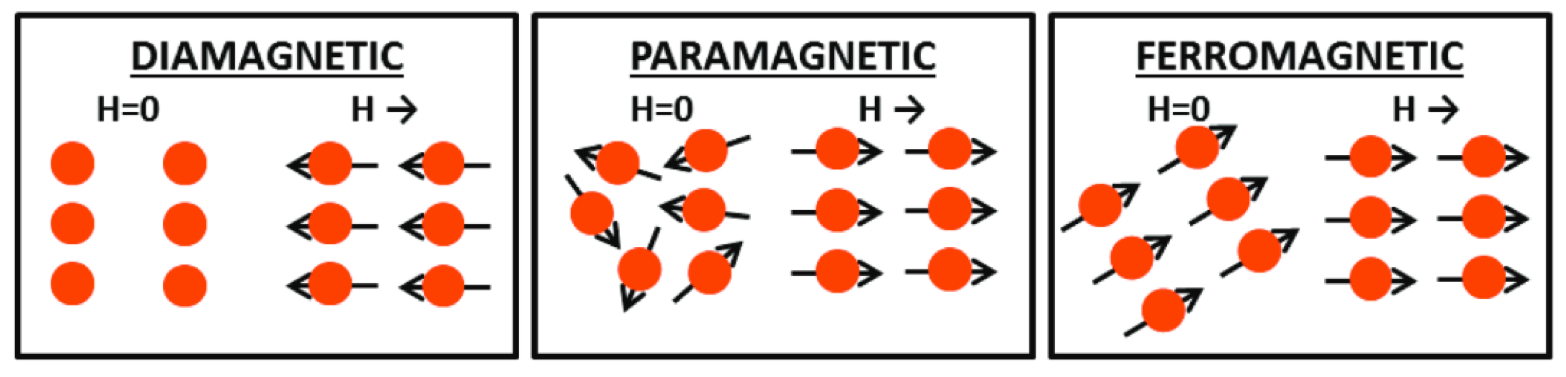
\includegraphics[width=0.7\linewidth]{Figures/Magnetics/ParaDiaFerro_Lacovacci2016.png}
  
    \tiny[Lacovacci2016]

    \vspace{0.24cm}
    
    \normalsize Ferromagnetism
    \small 
    \begin{itemize}
      \item Material exhibits \alert{pre-existing} dipoles which are oriented in domains with strong coupling.
      \item Domains align and \alert{strongly reinforce} external field ($\chi >> 0$). 
      \item Effect can be maintained if external field is removed.
      \item Examples: iron, nickel, ...
    \end{itemize}
    
  \end{center}
\end{frame}


\begin{frame}
  \begin{PointSix}{Temperature dependency}
    $$
      \chi = \frac{M}{H} = \frac{C}{T}
    $$
    \small
    \begin{itemize}
      \item $C$ is the Curie Constant.
      \item Overall, magnetic susceptibility decreases with increasing temperature.
    \end{itemize}
  \end{PointSix}
\end{frame}

\begin{frame}
  \begin{PointSix}{Temperature dependency}
    $$
      \chi \sim  \frac{1}{T - T_c}
    $$
    \small
    \begin{itemize}
      \item At the Curie Temperature materials loose their permanent magnetic properties.
    \end{itemize}
  \end{PointSix}
\end{frame}


\begin{frame}
  \begin{PointSix}{Learning Goals}
    \alert{Learning goals today:}
    \begin{itemize}
      \item Understand the shape of the magnetic anomalies
      \item Understand the measurement principle and sensors
      \item Understand different types of magnetism and its temperature dependency
    \end{itemize}
  \end{PointSix}
\end{frame}

